\subsection{Parametrische Darstellung}
Den Frequenzgang erhält man indem man die komplexe Variable $s$ durch iOmega ($i\omega$) ersetzt. \\
Das ist gleichbedeutend mit einem Schnitt der komplexen Funktion $G(s)$ entlang der imaginären Achse.
Damit wird jeder Kreisfrequenz $\omega$ eine komplexe Zahl $G(i\omega)$ zugeordnet. 
\\
\\
Bedingt durch den Schnitt hat der Frequenzgang eine geringere Aussagekraft als die Übertragungsfunktion. 
Die Bedeutung des Frequenzgangs ergibt sich aus der Tatsache, dass das stationäre Verhalten des Systems auf eine sinuidale Anregung beschrieben wird.\\
\\

Sei $u(t) = sin(\omega t)$, so ist $y_{stat}(\dot{t})$ %TODO: KONTROLLE
, dh. das Ausgangssignal nach Abklingen der Anfangswerte durch:
\begin{equation*}
    y_{stat}(t)=A*|G(i\omega )|sin(\omega t + \phi (G(i\omega )))
\end{equation*}

gegeben. %TODO: KONTROLLE und Block
%Der Frequenzgang liefert formal weniger Aussagen als die Übertragungsfunktion, da er nicht alle $s$ betrachtet, sondern nur die $s$, die auf der imaginären Achse liegen.\\
%Experimentell könnte der Frequenzgang durch die folgende Simulink-Schaltung aufgenommen werden. 
%TODO: Schaltung einfügen
%Man stellt eine Frequenz ein und schaut am Ausgang die Amplitudenverstärkung und die Phasenverschiebung an. Hat der Eingangssinus die Amplitude 1, kann ich die Verstärkung am Ausgang direkt ablesen. Den erhaltenen Punkt trägt man in das Bode-Diagramm ein. Danach wiederholt man das Experiment mit einer anderen Frequenz. Hat man genügend Punkte, so verbindet man diese und erhält das Bode-Diagramm. Ebenso wie wir an den Verläufen der Sprungantwort auf die Differentialgleichung schließen konnten, können Experten aus den Verläufen des Bode-Diagramms auf den Frequenzgang (und damit auf die Übertragungsfunktion und damit auf die Differentialgleichung) schließen.\\
%Die Phasenverschiebung kann selbstverständlich auch mit Computeralgebra ausgerechnet werden.
\subsection{Nichtparametrische Darstellung}
Experimentell kann der Frequenzgang durch folgende Simulink Schaltung aufgenommen werden:
\begin{figure}[H]
    \centering
    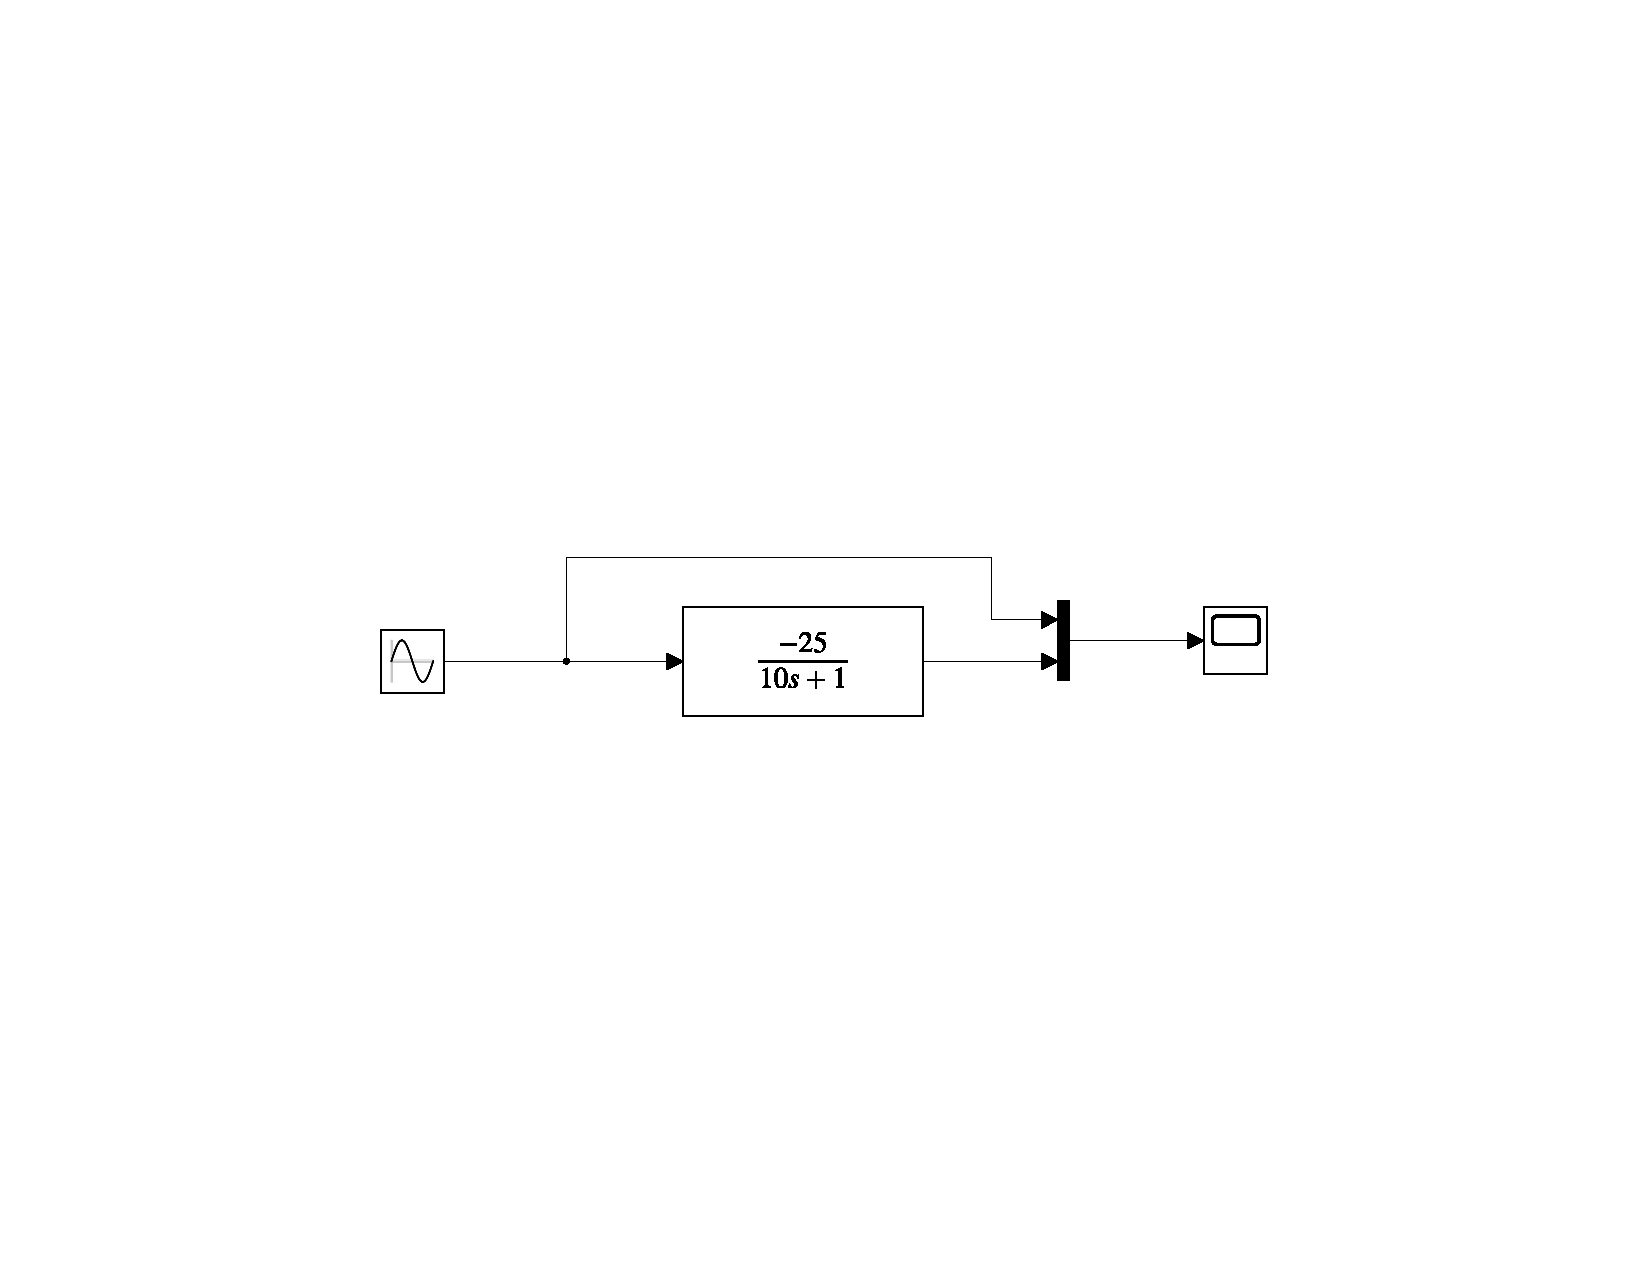
\includegraphics[width=8cm]{image/FrequenzgangSchaltung.pdf}
    \caption{Frequenzgang: Simulink Schaltung}
\end{figure}
\begin{figure}[H]
    \centering
    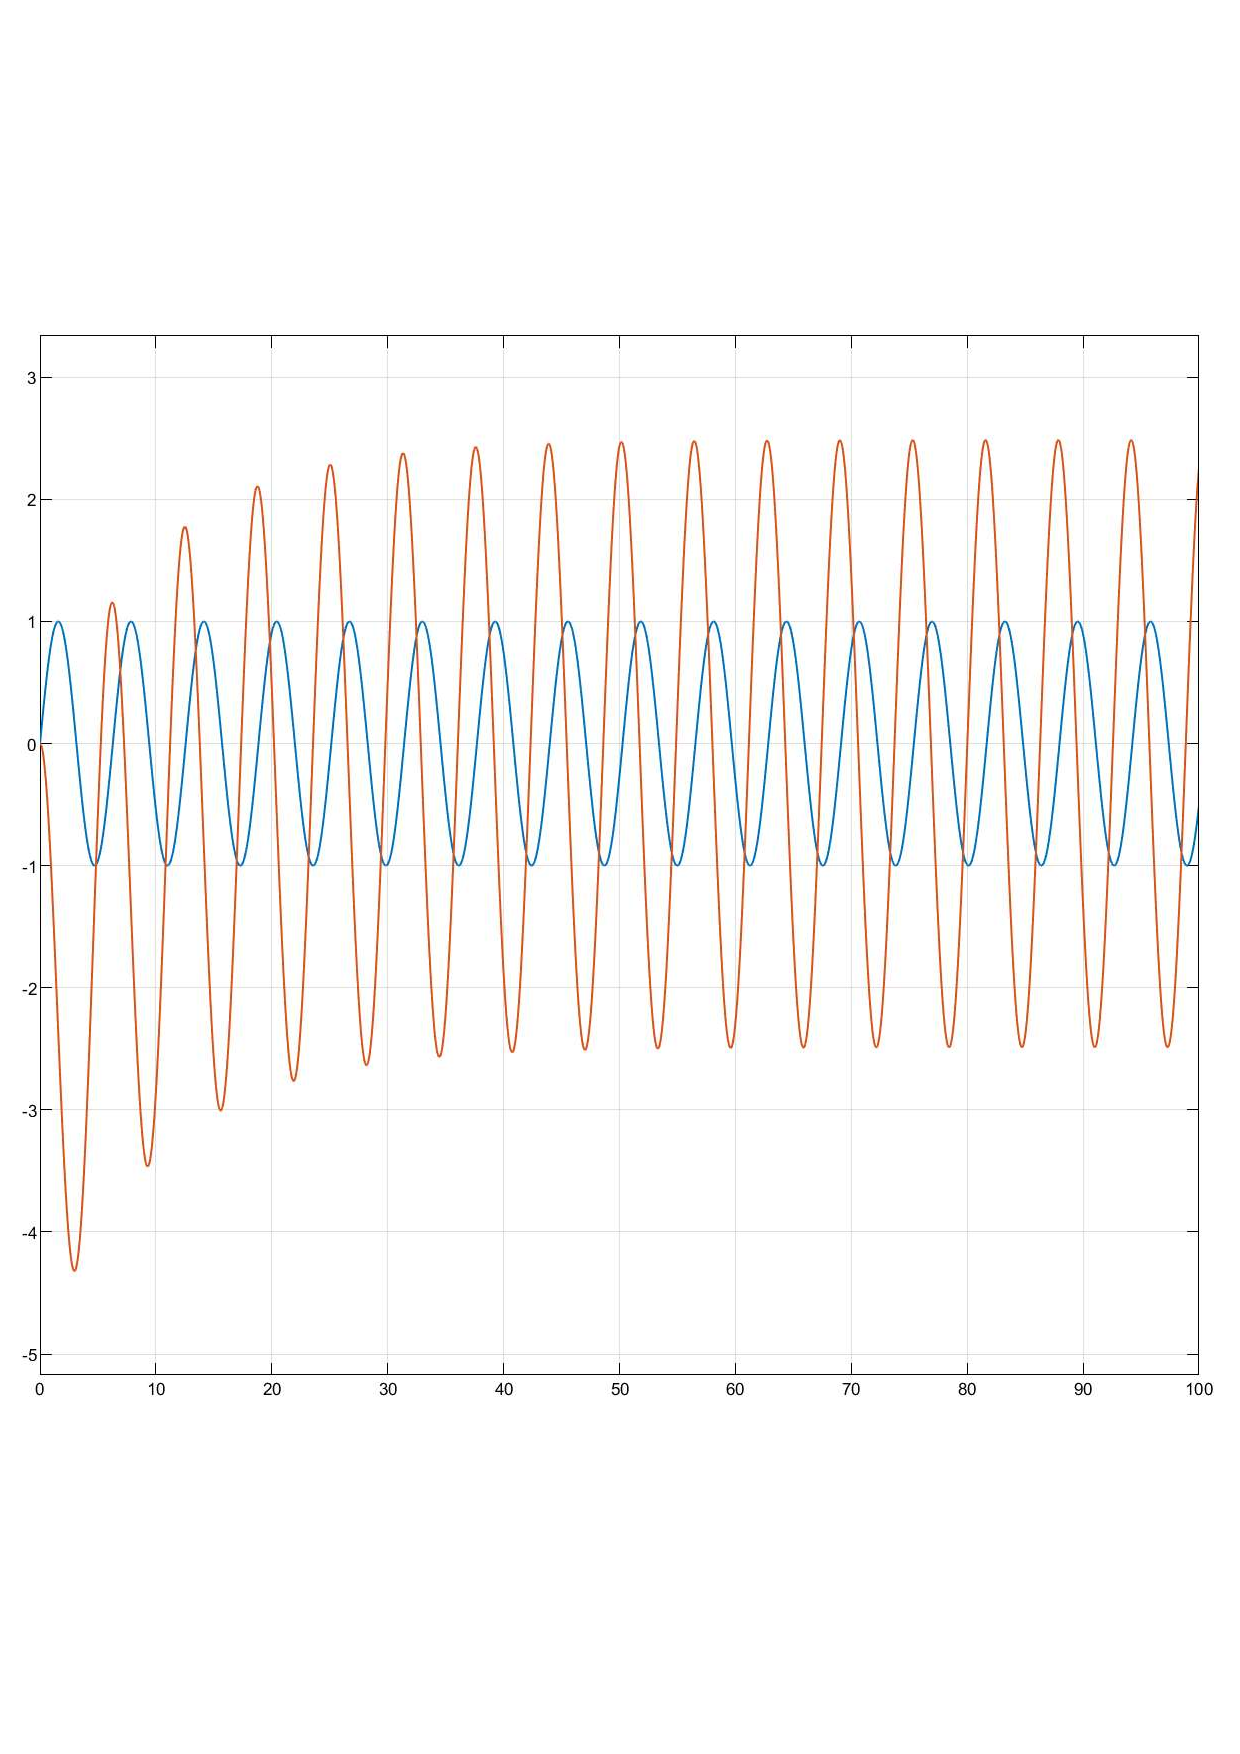
\includegraphics[width=8cm]{image/FrequenzgangAusgang.pdf}
    \caption{Frequenzgang: Plot mit Simulink}
\end{figure}

Am Eingangssinus wird eine Frequenz eingestellt und am Ausgang die Amplituden-
Verstärkung und die Phasenverschiebung betrachtet.
Hat der Eingang die Amplitude 1, kann man die AusgangsverstÄrkung direkt
ablesen.
Das Experiment wird mit verschiedenen Frequenz wiederholt und die jeweiligen
Ergebnisse werden dabei als Punkte in die folgenden Diagramme eingetragen.
\subsubsection{Nyquist-Plot (Ortskurve)}
Beim Nyquist-Plot ist auf der X-Achse der Realteil der gemessenen Punkte
und auf der Y-Achse der Imaginärteil, bei steigender Frequenz $\omega$ zu sehen.
Dieser lässt sich in Matlab mit folgendem Befehl generieren:\\
\texttt{nyquist(sys)}
\begin{figure}[H]
    \centering
    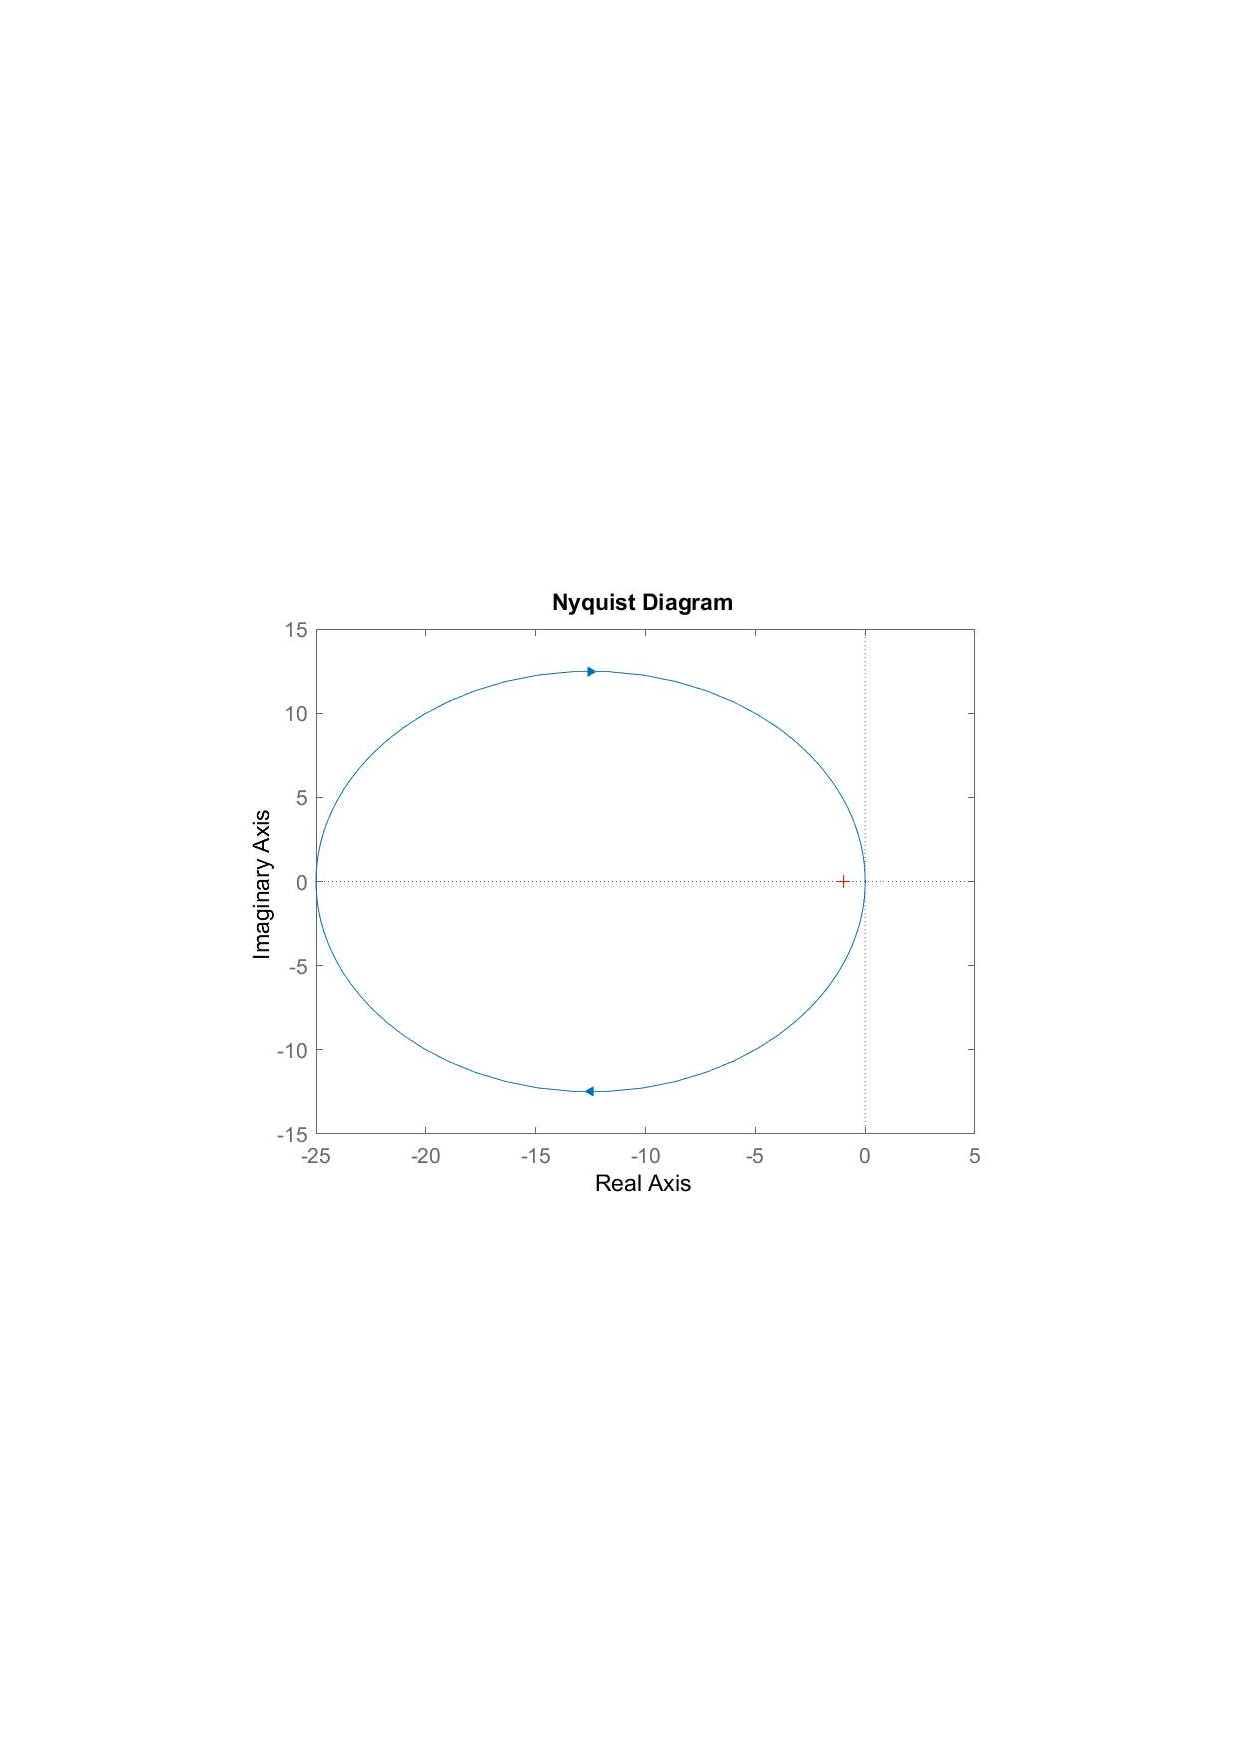
\includegraphics[width=8cm]{image/NyquistPlot.pdf}
    \caption{Frequenzgang: Nyquist Plot}
\end{figure}
\subsubsection{Bode-Plot}
In Matlab lässt sich der Bode Plot mit dem Befehl\\
\texttt{bode(sys)}\\
erzeugen.
\begin{figure}[H]
    \centering
    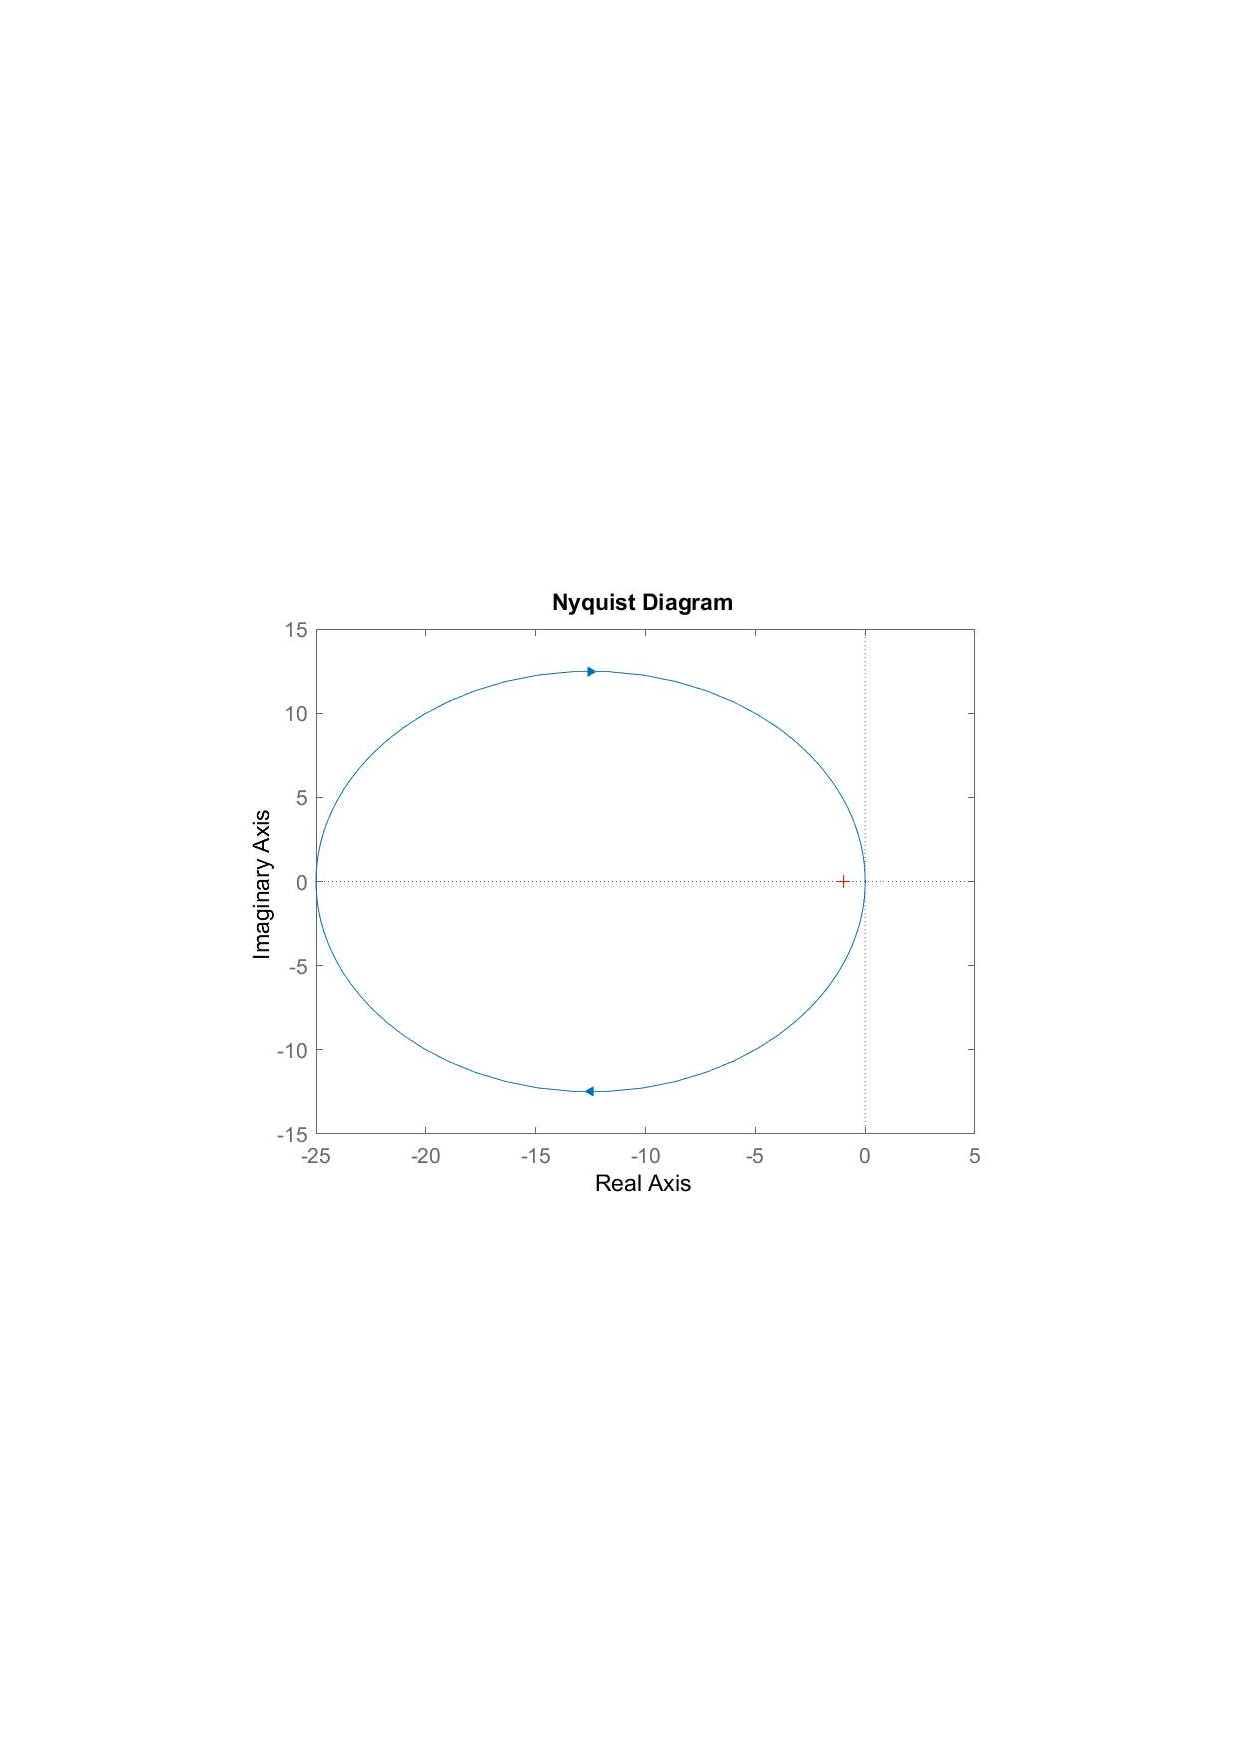
\includegraphics[width=8cm]{image/NyquistPlot.pdf}
    \caption{Frequenzgang: Bode-Plot}
\end{figure}